\documentclass[a4paper]{article}

\usepackage[utf8]{inputenc}
\usepackage[T1]{fontenc}
\usepackage{textcomp}
\usepackage[italian]{babel}
\usepackage{amsmath, amssymb}
\usepackage{siunitx}
\usepackage{caption}
\usepackage{graphicx}
\usepackage{subcaption}
\usepackage{booktabs} % Opzionale, per tabelle più belle se vuoi (\toprule, \midrule, \bottomrule)
\usepackage{ragged2e} % Per \Centering nelle minipage
\usepackage{float} % Per [htbp]
\usepackage{fullwidth}
\usepackage{darkmode}
%\enabledarkmode
\usepackage[margin=2cm]{geometry}

% ======================================================
% Impostazioni siunitx (opzionale, ma utile)
% ======================================================
\sisetup{
    output-decimal-marker = {,}, % Usa la virgola come separatore decimale
    uncertainty-mode = separate, % Mostra incertezza come ±
    separate-uncertainty = true, % Forza la separazione
    locale = IT, % Impostazioni locali italiane (es. per la virgola)
    group-digits = false % Evita di raggruppare le cifre (es. 10000 vs 10 000)
}

% ======================================================
% Appendice con le tabelle dati
% ======================================================
\usepackage{titling}
\usepackage{appendix}
\usepackage[colorlinks=true, linkcolor=blue, citecolor=blue, urlcolor=blue]{hyperref} % Per riferimenti cliccabili (opzionale ma utile)
\renewcommand{\appendixname}{Appendice} % Traduce "Appendix" in "Appendice"
\renewcommand{\appendixtocname}{Appendici} % Traduce "Appendices" nel ToC
\renewcommand{\appendixpagename}{Appendici} % Traduce "Appendices" nell'header/footer


\title{Microonde}
\author{Alessio Ramirez, Michele Rota, Sofia Zocchi}
\date{May 2025}

\begin{document}
\maketitle
\section{Caratterizzazione del fascio}
\subsection{Polarizzazione}
\subsubsection{Obiettivo}
Studiare la polarizzazione del fascio prodotto dall'emettitore e valutare la validità della Legge di Malus.

\subsubsection{Metodo}
Dal momento che l'emettitore produce un'onda polarizzata e il ricevitore si comporta come un filtro polarizzatore, è possibile osservare il segnale misurato al variare dell'angolo di cui è ruotato il ricevitore. Innanzitutto abbiamo disposto emettitore e ricevitore frontalmente, lungo lo stesso asse e a distanza fissata. Abbiamo quindi campionato al variare di $\alpha$, angolo tra la direzione di polarizzazione dell'onda e l'asse di trasmissione del filtro, i valori di tensione restituiti dal voltmetro collegato al ricevitore. Lo studio della dipendenza del segnale dal $cos(\alpha)$ è fondamentale per valutare se quanto restituito dal ricevitore risulta proporzionale al campo elettrico o all'intensità dell'onda. In quest'ultimo caso si ha la validità della Legge di Malus:
\begin{align}
I = I_0 cos^2(\alpha)
\label{eq:Legge di Malus}
\end{align}
Una volta raccolto i dati ne abbiamo quindi valutato l'accordo con la relazione \ref{eq:Legge di Malus}.

\subsubsection{Dati}
Abbiamo raccolto i valori di tensione misurati in seguito ad una rotazione del ricevitore attorno al proprio asse di un angolo $\alpha$ compreso tra $0^\circ$ e $180^\circ$, ogni $5^\circ$ \footnote{Tutti gli angoli misurati in gradi sono stati poi convertiti in radianti.}. Abbiamo considerato come errore sul valore di $\alpha$ la sensibilità del goniometro montato sul ricevitore, mentre, per quanto riguarda l'incertezza sul segnale, abbiamo osservato le fluttuazioni del valore di tensione restituito da voltmetro. Sono stati così misurati errori variabili, differenti da misura a misura, e corrispondenti a metà dell'intervallo entro cui oscillavano i valori di tensione.
Quanto misurato è visibile in tabella \ref{tab: dati Malus}.
\begin{table}[htbp]
\centering
\begin{tabular}{|c|c|}
\hline
$\alpha$ & tensione \\\hline\hline
0 ± 70 mrad & 2.97 ± 0.02 V \\
87 ± 70 mrad & 2.95 ± 0.02 V \\
175 ± 70 mrad & 2.90 ± 0.02 V \\
262 ± 70 mrad & 2.79 ± 0.01 V \\
349 ± 70 mrad & 2.67 ± 0.02 V \\
436 ± 70 mrad & 2.51 ± 0.02 V \\
524 ± 70 mrad & 2.33 ± 0.02 V \\
611 ± 70 mrad & 2.11 ± 0.01 V \\
698 ± 70 mrad & 1.92 ± 0.01 V \\
785 ± 70 mrad & 1.67 ± 0.02 V \\
873 ± 70 mrad & 1.42 ± 0.02 V \\
960 ± 70 mrad & 1.13 ± 0.01 V \\
1.05 ± 0.07 rad & 890 ± 10 mV \\
1.13 ± 0.07 rad & 580 ± 10 mV \\
1.22 ± 0.07 rad & 370 ± 10 mV \\
1.31 ± 0.07 rad & 190 ± 10 mV \\
1.40 ± 0.07 rad & 70 ± 10 mV \\
1.48 ± 0.07 rad & 20 ± 10 mV \\
1.57 ± 0.07 rad & 0 ± 10 mV \\
1.66 ± 0.07 rad & 30 ± 10 mV \\
1.75 ± 0.07 rad & 120 ± 10 mV \\
1.83 ± 0.07 rad & 270 ± 10 mV \\
1.92 ± 0.07 rad & 470 ± 10 mV \\
2.01 ± 0.07 rad & 720 ± 10 mV \\
2.09 ± 0.07 rad & 980 ± 10 mV \\
2.18 ± 0.07 rad & 1.26 ± 0.01 V \\
2.27 ± 0.07 rad & 1.52 ± 0.02 V \\
2.36 ± 0.07 rad & 1.75 ± 0.02 V \\
2.44 ± 0.07 rad & 2.00 ± 0.02 V \\
2.53 ± 0.07 rad & 2.24 ± 0.02 V \\
2.62 ± 0.07 rad & 2.45 ± 0.01 V \\
2.71 ± 0.07 rad & 2.65 ± 0.02 V \\
2.79 ± 0.07 rad & 2.81 ± 0.02 V \\
2.88 ± 0.07 rad & 2.89 ± 0.02 V \\
2.97 ± 0.07 rad & 2.93 ± 0.03 V \\
3.05 ± 0.07 rad & 2.96 ± 0.02 V \\
3.14 ± 0.07 rad & 2.97 ± 0.02 V \\
\hline
\end{tabular}
\caption{Dati sperimentali Legge di Malus}
\label{tab: dati Malus}
\end{table}

\subsubsection{Analisi dati}
\begin{figure}[htbp]
	\centering
	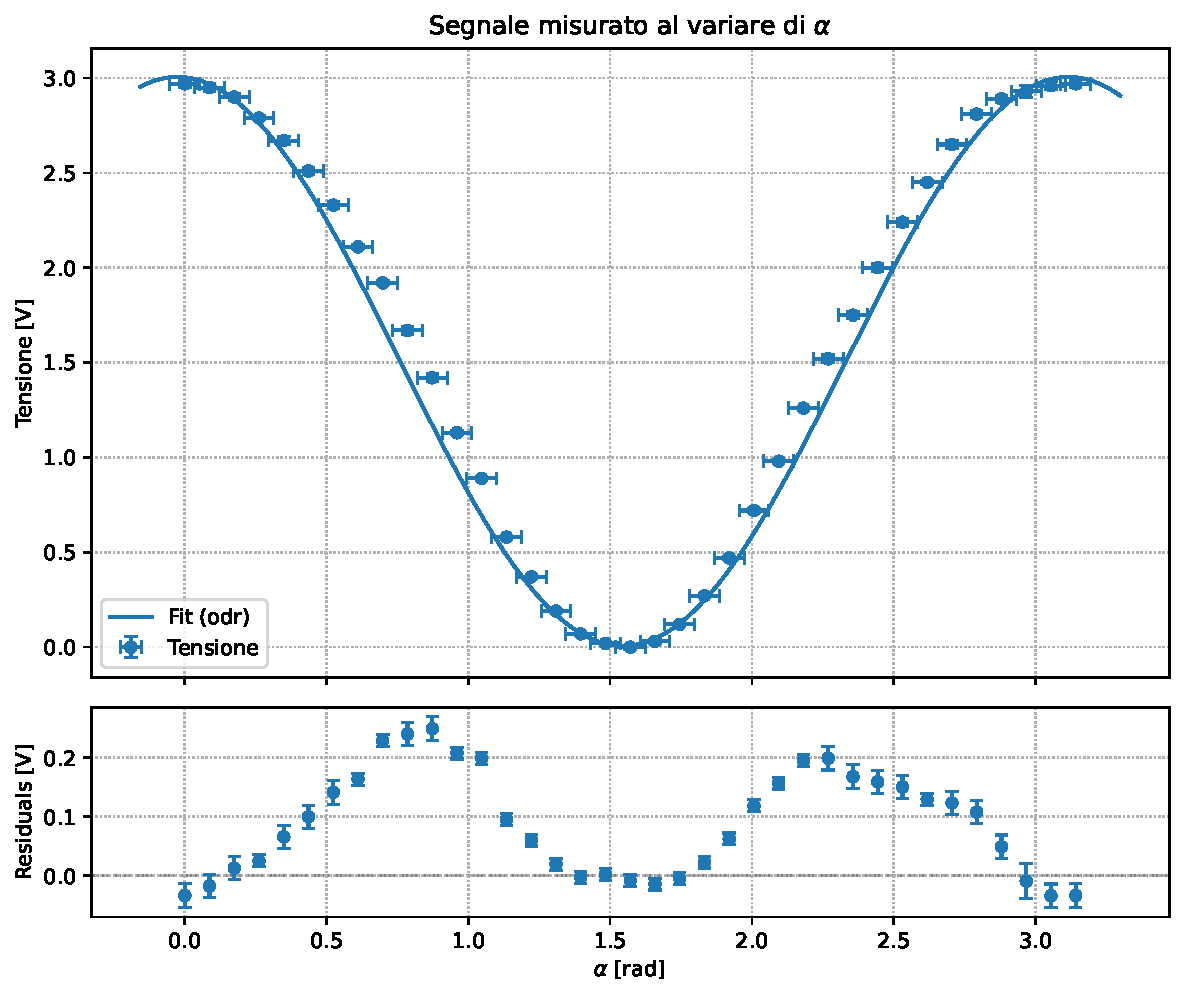
\includegraphics[width=0.7\textwidth]{grafici/Malus.pdf}
	\caption{Segnale misurato al variare dell'inclinazione del filtro polarizzatore}
	\label{Malus}
\end{figure}
Quanto misurato è stato utilizzato per verificare la validità di Malus. Abbiamo quindi effettuato un fit dei dati utilizzando una relazione della forma $V = k+V_0cos^2(\alpha)$, scelta sulla base di quanto descritto dalle legge \ref{eq:Legge di Malus} e nell'ipotesi il segnale di tensione fosse proporzionale all'intensità della radiazione. Nel realizzare l'interpolazione abbiamo considerato anche la presenza di un offset verticale $k$ dal momento che la lettura fatta dal ricevitore non è riferita ad una scala assoluta, ma anzi poteva essere traslata o amplificata utilizzando le apposite manopole. \footnote{Abbiamo provato ad interpolare i dati sperimentali anche utilizzando una legge della forma $V = k + V_0|cos(\alpha)|$, nell'ipotesi il segnale misurato fosse direttamente proporzionale al campo $E$ e non all'intensità $I$; i valori di chi quadro ricavati in tale configurazione dimostravano però un minore accordo.} I parametri del fit ottenuto mediante interpolazione sono raccolti in tabella \ref{fit.Malus}; il suo andamento è visualizzabile nel grafico \ref{Malus}.
\begin{table}[htbp]
\centering
\begin{tabular}{|l|ccccc|}
\hline
Risultati & k & $V_0$ & $\chi^2$ & DoF & $\chi^2/\nu$ \\\hline\hline
Fit Malus & 4.3 ± 7.6 m & 2.982 ± 0.013 & 24.8 & 35 & 0.707 \\\hline
\end{tabular}
\caption{Risultati fit Legge di Malus}
\label{fit.Malus}
\end{table}

\subsubsection{Conclusione}
Come si può osservare dall'esito positivo del test del chi quadro, i cui valori sono raccolti in tabella \ref{fit.Malus}, la Legge di Malus risulta verificata così come l'ipotesi che il segnale misurato dipenda dall'intensità dell'onda, in quanto proporzionale a $cos^2(\alpha)$.



\section{Angolo di Brewster}
\subsection{Obiettivo}
Osservare come il fenomeno della rifrazione sia influenzato dalla polarizzazione dell'onda elettromagnetica incidente. Valutare la radiazione trasmessa passando attraverso la superficie di separazione tra due mezzi, al variare dell'angolo di incidenza; ottenendo una stima dell'angolo di Brewster caratteristico della rifrazione aria-polietilene. 

\subsection{Metodo}
Poiché avevamo a disposizione una sorgente d'onda polarizzata ne abbiamo innanzitutto determinato la direzione di polarizzazione. Per fare ciò è stata montata tra emettitore e ricevitore un'apposita griglia metallica e, variandone la posizione, è stata individuata la condizione tale per cui il segnale misurato risultava nullo, deducendo quindi informazioni sulla polarizzazione dell'onda in esame. Da tale osservazione abbiamo ricavato che disponendo emettitore, e quindi anche ricevitore, con il lato più corto parallelo al tavolo (configurazione 1) si aveva radiazione polarizzata parallelamente al piano di incidenza; viceversa ruotando l'emettitore (configurazione 2) si otteneva un segnale con polarizzazione perpendicolare al piano di incidenza. Ci attendiamo quindi di poter determinare una stima dell'angolo di Brewster \footnote{Se un'onda polarizzata incide su una superficie di separazione tra due mezzi con polarizzazione parallela al piano di incidenza l'intensità della radiazione riflessa e della radiazione trasmessa dipendono dall'angolo di incidenza. In particolare in corrispondenza dell'angolo di Brewster l'intensità dell'onda riflessa è nulla e di conseguenza quella dell'onda trasmessa è massima.} mediante l'utilizzo della prima configurazione.
Per osservare la variazione del segnale trasmesso correlata ad un diverso angolo di incidenza, abbiamo disposto sorgente e ricevitore frontalmente, a distanza fissa, e abbiamo ruotato gradualmente la lastra di polietilene posta tra i due. Ciò è stato possibile in quanto la lastra si poteva montare su di un goniometro che ne misurava quindi facilmente la rotazione. A tale rotazione corrispondeva sia una variazione dell'angolo di incidenza durante la rifrazione aria-polietilene (onda in entrata nella lastra) che durante la rifrazione polietilene-aria (onda in uscita dalla lastra). L'informazione raccolta infatti dal ricevitore, e osservata sotto forma di tensione sul display del voltmetro, era correlata a un doppio fenomeno di rifrazione, tale per cui l'onda trasmessa ritornava in asse con l'onda incidente e quindi con la congiungente emettitore-ricevitore. 

\subsection{Dati}
Al fine di studiare l'intensità dell'onda trasmessa e la sua correlazione con l'angolo di incidenza abbiamo misurato il segnale recepito dal ricevitore al variare dell'inclinazione della lastra di polietilene. Quest'ultima è stata ruotata di $5^\circ$ alla volta. Il segnale osservato è stato misurato come tensione, quindi in Volt. Gli angoli riportati corrispondono invece all'angolo formato dalla perpendicolare alla lastra con la direzione della radiazione incidente, diretta lungo l'asse emettitore-trasmettitore. Per quanto riguarda la stima delle incertezze abbiamo considerato fisso l'errore sull'angolo di incidenza, pari alla sensibilità del goniometro: $\delta_{theta}=2^\circ$. Per le tensioni invece abbiamo valutato come oscillava il segnale restituito dal voltmetro, ottenendo errori variabili, corrispondenti a metà dell'intervallo di oscillazione. Quanto misurato per ciascuna direzione di polarizzazione è riportato nelle tabelle \ref{tab:brewster1} e \ref{tab:brewster2}.

\begin{table}[htbp]
\centering
\begin{tabular}{|c|c|}
\hline
$\theta$ & tensione \\\hline\hline
0 ± 30 mrad & 2.47 ± 0.01 V \\
87 ± 30 mrad & 2.46 ± 0.01 V \\
175 ± 30 mrad & 2.54 ± 0.01 V \\
262 ± 30 mrad & 2.59 ± 0.01 V \\
349 ± 30 mrad & 2.54 ± 0.01 V \\
436 ± 30 mrad & 2.55 ± 0.02 V \\
524 ± 30 mrad & 2.52 ± 0.01 V \\
611 ± 30 mrad & 2.68 ± 0.01 V \\
698 ± 30 mrad & 3.02 ± 0.01 V \\
785 ± 30 mrad & 3.62 ± 0.01 V \\
873 ± 30 mrad & 4.34 ± 0.01 V \\
960 ± 30 mrad & 4.66 ± 0.01 V \\
1.05 ± 0.03 rad & 4.45 ± 0.01 V \\
1.13 ± 0.03 rad & 3.00 ± 0.01 V \\
1.22 ± 0.03 rad & 1.58 ± 0.01 V \\
\hline
\end{tabular}
\caption{Dati trasmissione con polarizzazione parallela al piano di incidenza}
\label{tab:brewster1}
\end{table}

\begin{table}[htbp]
\centering
\begin{tabular}{|c|c|}
\hline
$\theta$ & tensione \\\hline\hline
0 ± 30 mrad & 2.50 ± 0.01 V \\
87 ± 30 mrad & 2.55 ± 0.01 V \\
175 ± 30 mrad & 2.84 ± 0.01 V \\
262 ± 30 mrad & 2.90 ± 0.01 V \\
349 ± 30 mrad & 2.76 ± 0.01 V \\
436 ± 30 mrad & 2.66 ± 0.01 V \\
524 ± 30 mrad & 2.65 ± 0.01 V \\
611 ± 30 mrad & 2.52 ± 0.01 V \\
698 ± 30 mrad & 2.56 ± 0.01 V \\
785 ± 30 mrad & 2.71 ± 0.02 V \\
873 ± 30 mrad & 2.86 ± 0.02 V \\
960 ± 30 mrad & 3.17 ± 0.02 V \\
1.05 ± 0.03 rad & 2.64 ± 0.02 V \\
\hline
\end{tabular}
\caption{Dati trasmissione con polarizzazione perpendicolare al piano di incidenza}
\label{tab:brewster2}
\end{table}

\subsection{Analisi dati}
\begin{figure}[htbp]
	\centering
	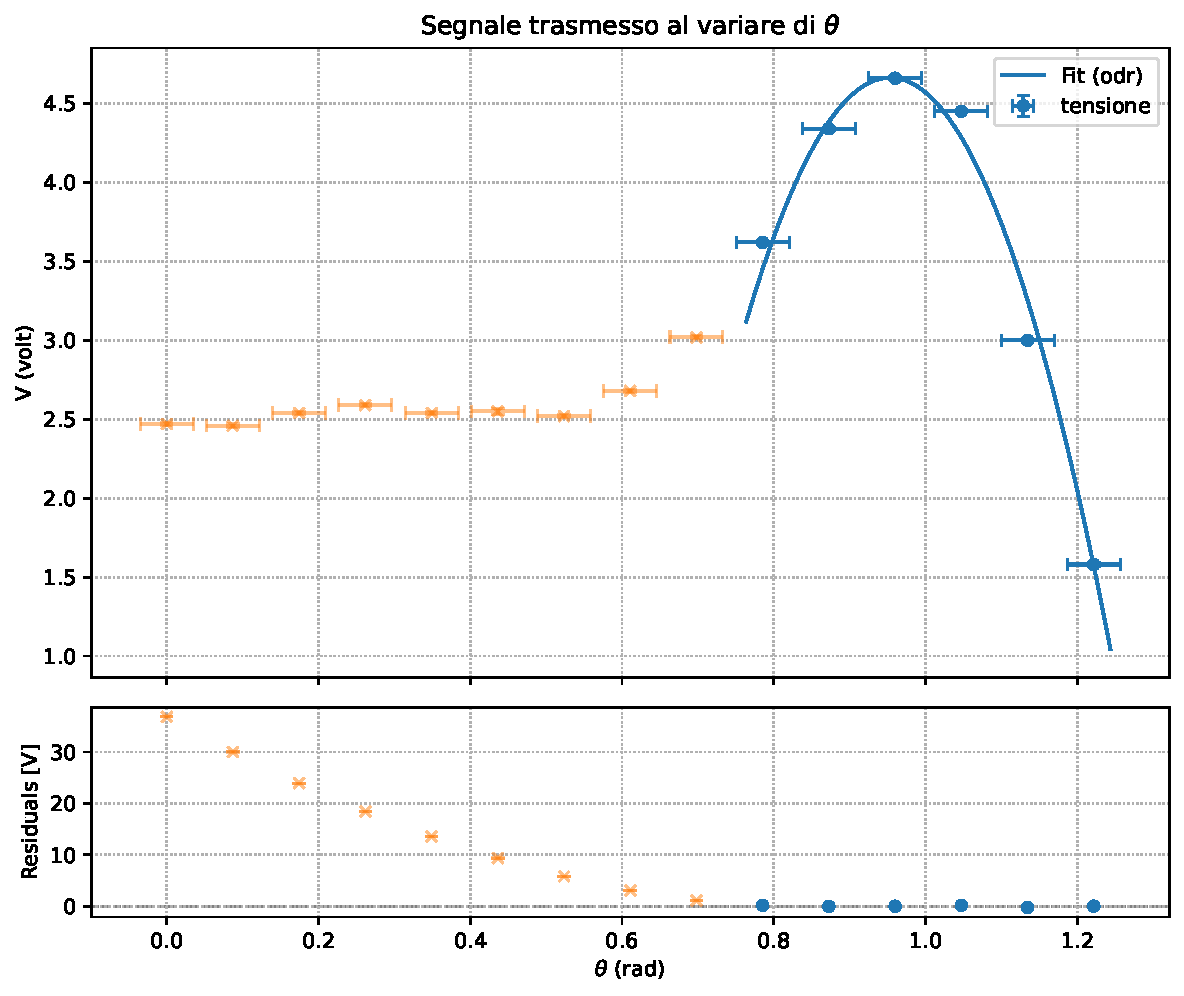
\includegraphics[width=0.8\textwidth]{grafici/brewster.pdf}
	\caption{Onda trasmessa con polarizzazione parallela al piano di incidenza}
	\label{Brewster1}
\end{figure}
\begin{figure}[htbp]
	\centering
	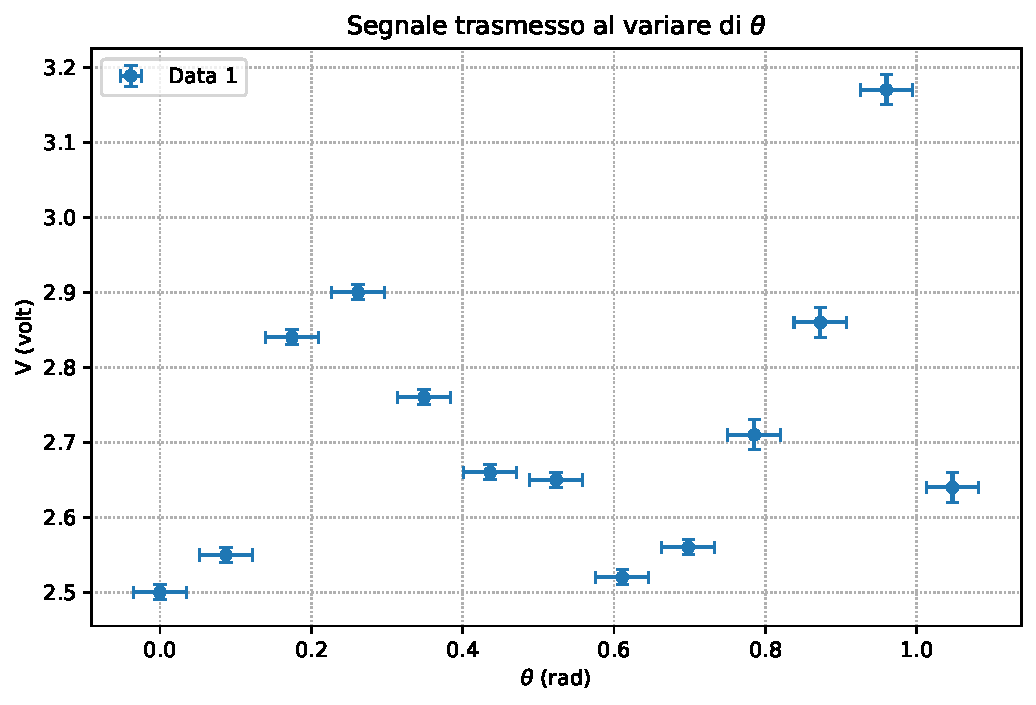
\includegraphics[width=0.8\textwidth]{grafici/brewster1.pdf}
	\caption{Onda trasmessa con polarizzazione perpendicolare al piano di incidenza}
	\label{Brewster2}
\end{figure}

L'andamento del segnale ricevuto al variare di $\theta$ con polarizzazione parallela al piano di incidenza è visualizzabile nel grafico \ref{Brewster1}. Il massimo del segnale trasmesso si ha in corrispondenza dell'angolo di Brewster, il cui valore è stato ottenuto attuando un'interpolazione parabolica con i punti campionati in prossimità del massimo. Si è utilizzata una relazione del tipo $y = ax^2 + bx +c$, con $y= V$ e $x=\theta$, da cui si sono ricavati $a, b, c$ e i relativi errori, poi utilizzati per determinare la posizione del massimo. Più precisamente:
\begin{align}
  \theta_{B} = -\frac{b}{2a} \qquad & \text{,}\qquad
  \delta_{\theta_{B}} = \sqrt{(\frac{-2}{a}\delta_b)^2 +(\frac{2b}{a^2}\delta_a)^2}. \label{eq:angolo brewster}
\end{align}
In tabella \ref{tab:fit.brewster} sono raccolti i valori dei parametri di fit e la stima dell'angolo di Brewster.
\begin{table}[htbp]
\centering
\begin{tabular}{|l|ccccccc|}
\hline
Risultati & a & b & c & $\chi^2$ & DoF & $\chi^2/\nu$ & $\theta_B$ [$^\circ$]\\\hline\hline
Fit Brewster & -42.9 ± 4.3 & 81.9 ± 8.4 & -34.4 ± 4.1 & 0.803 & 3 & 0.268 & 54.69 ± 7.84 \\\hline
\end{tabular}
\caption{Risultati fit angolo di Brewster}
\label{tab:fit.brewster}
\end{table}
Per quanto riguarda invece le misurazioni effettuate con polarizzazione perpendicolare al piano di incidenza, come è possibile osservare dal grafico \ref{Brewster2}, si è osservato un segnale oscillante al variare di $\theta$. Inoltre ponendosi più volte in corrispondenza dello stesso angolo si potevano misurare valori di tensione differenti. Abbiamo quindi interpretato quanto misurato come segnale di fondo. Tale ipotesi deriva anche dal fatto che le tensioni misurate con polarizzazione perpendicolare al piano di incidenza assumevano valori compresi tra $2.5V$ e $3V$, compatibili con il plateau iniziale rilevato per polarizzazione parallela al piano di incidenza.

\subsection{Conclusione}
Il valore dell'angolo di Brewster ricavato sperimentalmente è stato infine confrontato con quanto atteso. Se si ha passaggio di un'onda elettromagnetica da un mezzo con indice di rifrazione minore ad uno con indice di rifrazione maggiore, come avviene durante l'ingresso dell'onda nella lastra, l'angolo di Brewster risulta pari a $\theta_B = arctg(\frac{n_2}{n_1})$, dove $n_1 = 1$ indica l'indice di rifrazione dell'aria, mentre $n_2 \approx 1.5$ corrisponde all'indice di rifrazione del polietilene. Il confronto tra $\theta_{s}$ e $\theta_{att}$ è stato realizzato mediante z-test, con $z = \frac{\theta_s - \theta_{att}}{\delta_{\theta}}$. I suoi risultati sono riportati in tabella \ref{tab:brewster_compatibilita}. Seppur sia presente accordo tra quanto misurato e quanto atteso è importante sottolineare che il segnale studiato non corrispondeva esattamente al segnale trasmesso in seguito al passaggio aria-polietilene, ma alla somma del segnale trasmesso per onda in entrata e in uscita dalla lastra di polietilene.
\begin{table}[htbp] 
\centering
\begin{tabular}{|l|c|}
\hline
$\theta_{att} [^\circ]$ & Probabilità entro t sigma \\
\hline
56.31 & 0.58 \\
\hline
\end{tabular}
\caption{Risultati del test di compatibilità tra $\theta_s$ e $\theta_{att}$.}
\label{tab:brewster_compatibilita}
\end{table}


\section{Diffrazione di Bragg}
\subsection{Obiettivo}
\begin{figure}[htbp]
	\centering
	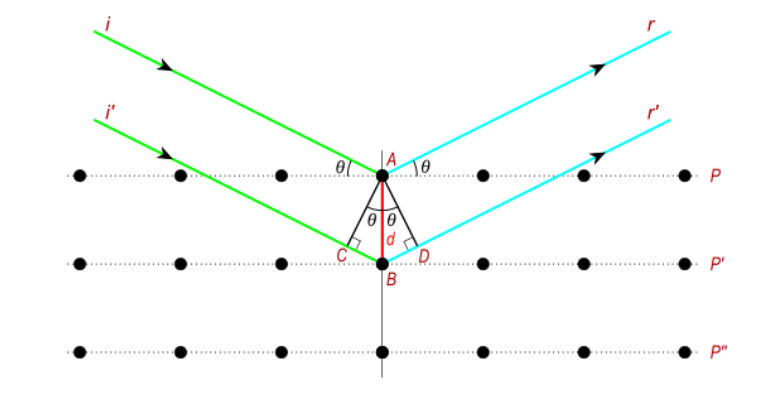
\includegraphics[width=0.5\textwidth]{grafici/schema.bragg.png}
	\caption{Reticolo di Bragg}
	\label{schema.bragg}
\end{figure}

Verificare empiricamente la Legge di Bragg. Utilizzare un cubo realizzato in materiale plastico con incastonate all'interno sferette d'acciaio, atto a  riprodurre in scala macroscopica la struttura reticolare di un cristallo. Studiare l'interferenza dovuta all'interazione tra i raggi riflessi dai diversi piani paralleli al piano reticolare (cioè dalle diverse file di sferette, come schematizzato in figura \ref{schema.bragg}) al variare dell'angolo $\theta$ di incidenza del fascio.

\subsection{Metodo}
\begin{figure}[htbp]
	\centering
	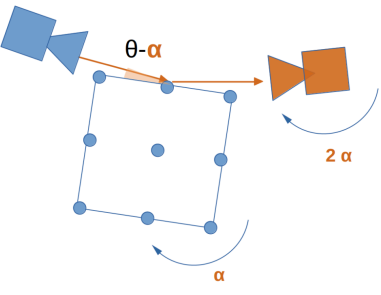
\includegraphics[width=0.4\textwidth]{grafici/disposizione.bragg.png}
	\caption{Disposizione apparato sperimentale}
	\label{disposizione.bragg}
\end{figure}

Dopo aver posizionato il cubo di Bragg sul goniometro mediante l'utilizzo dell'apposito supporto, abbiamo disposto il ricevitore in modo tale che fosse possibile captare il segnale riflesso dal cubo. Per variare l'angolo di incidenza del fascio abbiamo lasciato fisso l'emettitore e ruotato gradualmente il cubo. Ad ogni rotazione di un angolo $\alpha$ in senso orario del cubo seguiva una rotazione in senso orario di un angolo $2\alpha$ del ricevitore, come si può osservare in figura \ref{disposizione.bragg}, \footnote{Lo stesso ragionamento vale per rotazioni in senso antiorario} in modo tale che il ricevitore puntasse nella direzione del raggio riflesso, dal momento che $\theta_{incidente} = \theta_{riflesso}$. Misuravamo quindi il segnale acquisito dal ricevitore ad ogni rotazione. Tale procedura ci ha permesso però di osservare l'andamento del segnale soltanto parzialmente, in quanto siamo riusciti a campionare un numero limitato di angoli $\alpha$, poiché dovevamo mantenere una posizione reciproca tra ricevitore ed emettitore tale per cui il segnale prodotto non arrivasse direttamente al ricevitore senza prima incidere sul cubo.

\subsection{Dati}
Riportiamo nella tabella \ref{tab:bragg} l'intensità del segnale misurato in corrispondenza degli angoli di rotazione considerati, definiti rispetto 
alla congiungente con l'emettitore.
Abbiamo stimato l'incertezza sul segnale, misurato come tensione, valutando l'oscillazione di quest'ultimo, scegliendo cioè come errore metà dell'intervallo di valori restituiti dal voltmetro. Per quanto riguarda invece l'incertezza sull'angolo di rotazione abbiamo fissato $\delta_{theta}=2^\circ$, corrispondente all'angolo intercettato dalla punta del goniometro e cioè alla sensibilità dello strumento.

\begin{table}[htbp]
\centering
\begin{tabular}{|c|c|}
\hline
$\theta$ & tensione \\\hline\hline
349 ± 30 mrad & 30 ± 10 mV \\
401 ± 30 mrad & 30 ± 10 mV \\
436 ± 30 mrad & 30 ± 10 mV \\
471 ± 30 mrad & 40 ± 20 mV \\
524 ± 30 mrad & 90 ± 10 mV \\
559 ± 30 mrad & 180 ± 20 mV \\
611 ± 30 mrad & 210 ± 20 mV \\
663 ± 30 mrad & 230 ± 10 mV \\
698 ± 30 mrad & 280 ± 10 mV \\
750 ± 30 mrad & 320 ± 10 mV \\
785 ± 30 mrad & 300 ± 20 mV \\
838 ± 30 mrad & 150 ± 10 mV \\
873 ± 30 mrad & 140 ± 10 mV \\
960 ± 30 mrad & 20 ± 10 mV \\
1.05 ± 0.03 rad & 50 ± 10 mV \\
\hline
\end{tabular}
\caption{Dati sperimentali cubo di Bragg}
\label{tab:bragg}
\end{table}

\subsection{Analisi dati}
\begin{figure}[htbp]
	\centering
	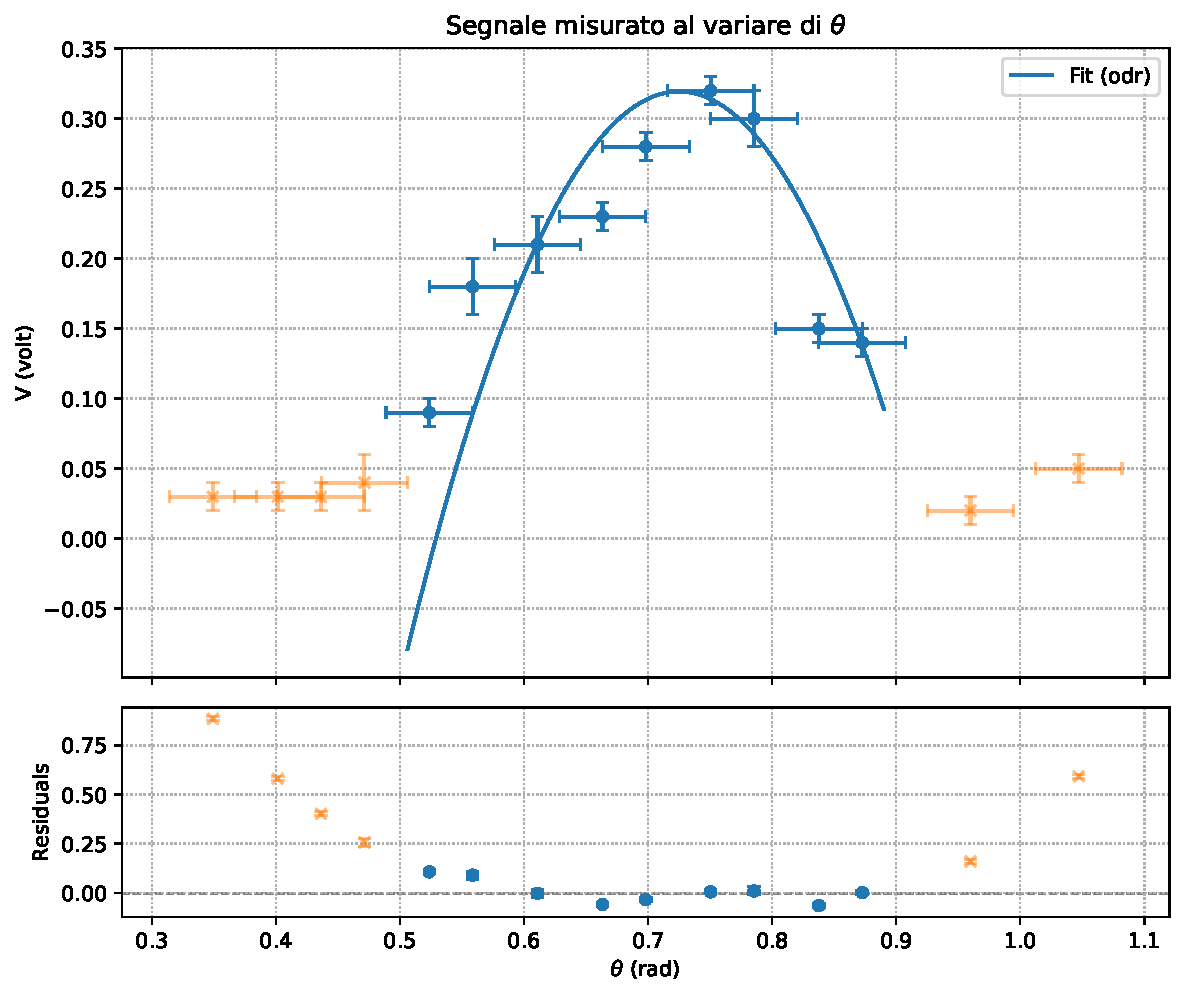
\includegraphics[width=0.8\textwidth]{grafici/bragg.pdf}
	\caption{Diffrazione cubo di Bragg}
	\label{dati.bragg}
\end{figure}
La Legge di Bragg descrive la posizione dei massimi di interferenza, i quali si hanno in corrispondenza di $\theta$, angolo formato dal raggio incidente con il piano reticolare scelto, tale per cui vale la relazione:
\begin{align}
    n\lambda=2d sin(\theta)
    \label{eq:bragg} 
\end{align}
in cui $n$ indica l'ordine del massimo ed è quindi un numero intero, $\lambda$ è la lunghezza d'onda del raggio e $d$ corrisponde alla distanza tra due piani di sferette distinti. Nel caso in esame abbiamo misurato $d = (3.8 \pm 0.1)cm$.
Valutando l'andamento del segnale misurato al variare dell'angolo, visualizzabile in figura \ref{dati.bragg}, abbiamo stimato la posizione del massimo di interferenza. Tale stima è stata ricavata utilizzando un'interpolazione parabolica applicata ai punti centrali del grafico. Abbiamo quindi utilizzando una legge della forma $y = ax^2 + bx +c$, con $y= V$ e $x=\theta$, a partire dalla quale abbiamo stimato i valori dei parametri $a, b, c$ e i relativi errori, poi utilizzati per ricavare la posizione del vertice. Più precisamente abbiamo ricavato l'angolo per cui il segnale è massimo dalla relazione $\theta_{\text{max}} = -\frac{b}{2a}$, con errore $\delta_{theta_{\text{max}}} = \sqrt{(\frac{-2}{a}\delta_b)^2 +(\frac{2b}{a^2}\delta_a)^2}$. Tale risultato ci ha permesso di ricavare la lunghezza d'onda della radiazione; invertendo la \ref{eq:bragg} e utilizzando la propagazione degli errori si ottiene\footnote{Si è ipotizzato di trovarsi in corrispondenza del primo massimo, cioè $n=1$}:
\begin{align}
  \lambda_s &= \frac{2d \sin(\theta_{\text{max}})}{n} \qquad & \text{,}\qquad
  \delta \lambda_s = \sqrt{\delta \theta_{\text{max}}^2 ( \frac{2d \cos(\theta_{\text{max}})}{n})^2 + \delta_d^2 (\frac{2sin(\theta_{\text{max}})}{n})^2}. \label{eq:lunghezza_bragg}
\end{align}
I risultati ricavati sono riportati nella tabella \ref{tab:fit.bragg}.
\begin{table}[htbp]
\centering
\begin{tabular}{|l|ccccccc|}
\hline
Risultati & a & b & c & $\chi^2$ & DoF & $\chi^2/\nu$ & $\lambda_s [m]$  \\\hline\hline
Fit massimo & -8.3 ± 2.0 & 12.1 ± 2.8 & -4.0 ± 1.0 & 5.78 & 6 & 0.963 & 0.051 ±0.014\\\hline
\end{tabular}
\caption{Risultati fit cubo di Bragg}
\label{tab:fit.bragg}
\end{table}

\subsection{Conclusione}
Vogliamo sottolineare come l'andamento del segnale al variare dell'angolo non sia regolare, come è possibile osservare dalle misure riportate in figura \ref {dati.bragg}. Tale irregolarità è da imputarsi agli effetti di bordo dovuti alla struttura di ricevitore e trasmettitore, ma anche ai vari fattori di rumore esterno, quali la presenza di dispositivi elettronici nei pressi della strumentazione o l'attività degli apparati sperimentali circostanti. Nel corso dell'esperienza abbiamo infatti potuto osservare come il segnale misurato dal voltmetro oscillasse anche a causa di fattori esterni. Ne consegue che abbiamo ottenuto una misura di $\lambda_s$ molto poco accurata, dal momento che presenta un errore relativo $\approx 27\%$.

\end{document}
